% Figure 1 of terminalbench_deck: image 1:1 Runtime 1:N session 1:1 microVM.
% Build: xelatex tb_fig01_cardinality.tex  (-> .pdf, included by ../terminalbench_deck.md)
\documentclass[tikz,border=4pt]{standalone}
\usepackage{fontspec}
\setmainfont{DejaVu Sans}
\setmonofont{DejaVu Sans Mono}
\usetikzlibrary{positioning,arrows.meta,fit,backgrounds,calc}
\definecolor{img}{RGB}{230,230,230}
\definecolor{host}{RGB}{214,216,240}
\definecolor{ac}{RGB}{255,236,204}
\definecolor{vm}{RGB}{214,238,220}
\definecolor{ink}{RGB}{40,40,90}
\begin{document}
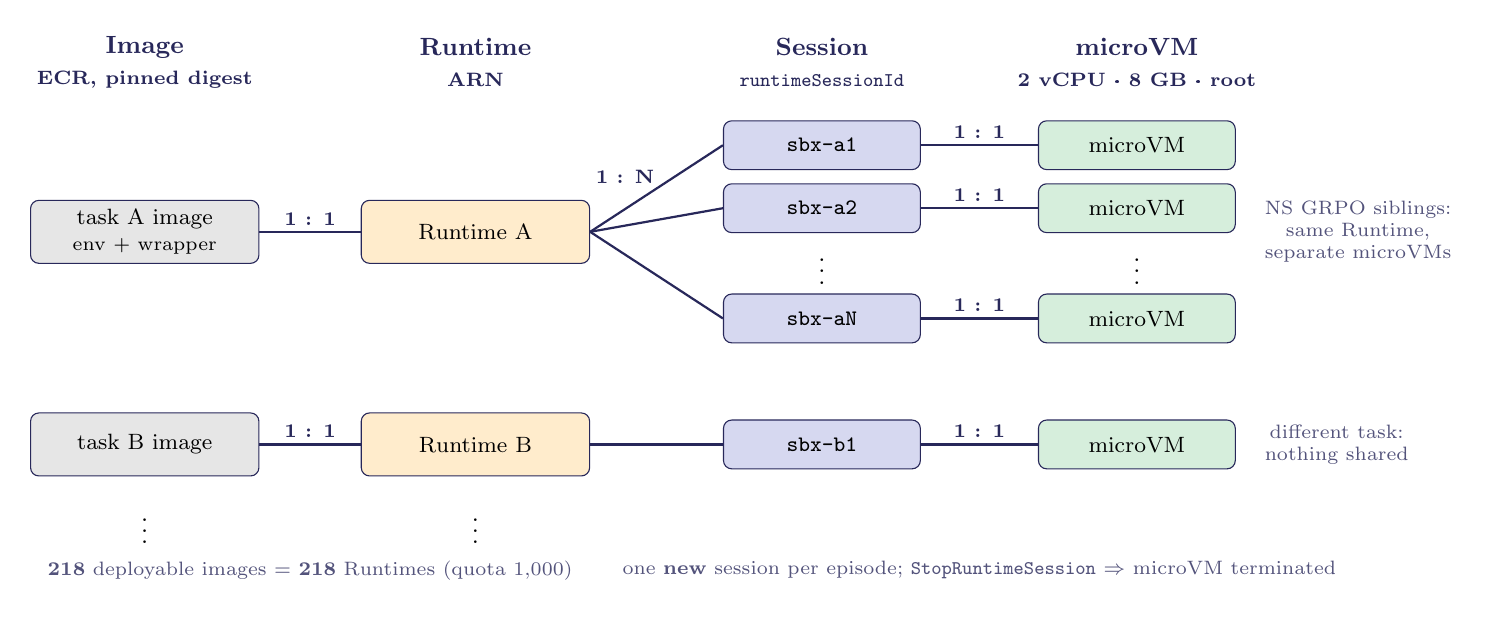
\begin{tikzpicture}[
  font=\footnotesize,
  box/.style={draw=ink, rounded corners=3pt, fill=#1, align=center, inner sep=3pt, minimum height=0.8cm, minimum width=2.9cm},
  sbox/.style={box=#1, minimum width=2.5cm, minimum height=0.62cm},
  line/.style={thick, draw=ink},
  card/.style={font=\scriptsize\bfseries, text=ink, fill=white, inner sep=1pt},
  head/.style={font=\small\bfseries, text=ink, align=center},
  note/.style={font=\scriptsize, text=ink!80, align=center},
]
% column heads
\node[head] at (0,1.25)  {Image\\\scriptsize ECR, pinned digest};
\node[head] at (4.2,1.25) {Runtime\\\scriptsize ARN};
\node[head] at (8.6,1.25) {Session\\\scriptsize \texttt{runtimeSessionId}};
\node[head] at (12.6,1.25) {microVM\\\scriptsize 2 vCPU · 8 GB · root};

% ---- task A: a GRPO group of NS episodes ----
\node[box=img] (ia) at (0,-0.9) {task A image\\\scriptsize env + wrapper};
\node[box=ac]  (ra) at (4.2,-0.9) {Runtime A};
\foreach \i/\y/\t in {1/0.2/\texttt{sbx-a1}, 2/-0.6/\texttt{sbx-a2}, 3/-2.0/\texttt{sbx-aN}} {
  \node[sbox=host] (sa\i) at (8.6,\y) {\t};
  \node[sbox=vm]   (va\i) at (12.6,\y) {microVM};
  \draw[line] (ra.east) -- (sa\i.west);
  \draw[line] (sa\i) -- node[card, above=1pt] {1 : 1} (va\i);
}
\node[font=\small] at (8.6,-1.3) {$\vdots$};
\node[font=\small] at (12.6,-1.3) {$\vdots$};
\draw[line] (ia) -- node[card, above=1pt] {1 : 1} (ra);
\node[card] at (6.1,-0.2) {1 : N};
\node[note, anchor=west] at (14.1,-0.9) {NS GRPO siblings:\\same Runtime,\\separate microVMs};

% ---- task B ----
\node[box=img] (ib) at (0,-3.6) {task B image};
\node[box=ac]  (rb) at (4.2,-3.6) {Runtime B};
\node[sbox=host] (sb1) at (8.6,-3.6) {\texttt{sbx-b1}};
\node[sbox=vm]   (vb1) at (12.6,-3.6) {microVM};
\draw[line] (ib) -- node[card, above=1pt] {1 : 1} (ra.west |- ib) -- (rb);
\draw[line] (rb) -- (sb1);
\draw[line] (sb1) -- node[card, above=1pt] {1 : 1} (vb1);
\node[note, anchor=west] at (14.1,-3.6) {different task:\\nothing shared};

\node[font=\small] at (0,-4.6) {$\vdots$};
\node[font=\small] at (4.2,-4.6) {$\vdots$};
\node[note] at (2.1,-5.2) {\textbf{218} deployable images = \textbf{218} Runtimes (quota 1,000)};
\node[note] at (10.6,-5.2) {one \textbf{new} session per episode; \texttt{StopRuntimeSession} $\Rightarrow$ microVM terminated};
\end{tikzpicture}
\end{document}
